% This is file JFM2esam.tex
% first release v1.0, 20th October 1996
%       release v1.01, 29th October 1996
%       release v1.1, 25th June 1997
%       release v2.0, 27th July 2004
%       release v3.0, 16th July 2014
%       release v4.0, 15th June 2017
%   (based on JFMsampl.tex v1.3 for LaTeX2.09)
% Copyright (C) 1996, 1997, 2014, 2017 Cambridge University Press

\documentclass[12pt]{RBM_P}
\usepackage{graphicx}
% \usepackage{epstopdf, epsfig}

\usepackage[utf8]{inputenc}
\usepackage[T1]{fontenc}
\usepackage{amsmath}
\usepackage{setspace}
\usepackage[a4paper, left=25mm, right=25mm, top=30mm, bottom=30mm]{geometry}
\usepackage[style=ieee]{biblatex}

\bibliography{reference.bib}

\newtheorem{lemma}{Lemma}
\newtheorem{corollary}{Corollary}

% \shorttitle{RBM Research Proposal}
% \shortauthor{A. N. Other, H.-C. Smith and J. Q. Public}

\title{Title of RBM Research Proposal}


% \author{Alan N. Other\aff{1}
%   \corresp{\email{jpp@damtp.cam.ac.uk}},
%   H. - C. Smith\aff{1}
%  \and J. Q.  Public\aff{2}}

% \affiliation{\aff{1}Plasma Physics Laboratory, University of America,
% Somewhere, IN 12345, USA
% \aff{2}Department of Physics, University of
% Camford, Academic Street, Camford CF3 5QL, UK}

\begin{document}


\newcommand{\GroupProjectTitle}{Your Group Project Title}
\newcommand{\SubProjectTitle}{Your Sub Project Title}

\newcommand{\StudentName}{First Name . Last Name}
\newcommand{\StudentID}{5000XXXX}
\newcommand{\Email}{your.id@connect.hkust-gz.edu.cn}
\newcommand{\Supervisor}{Lionel M. NI}
\newcommand{\HubThrust}{Info Hub / DSA Thrust}
\newcommand{\ProjectMentor}{Ke XUE}



\begin{titlepage}
    \begin{center}
        \vspace*{1cm}

        \huge
        \textbf{HKUST (GZ)}
        \vspace{0.5cm}

        \textbf{Master Thesis Proposal for MPhil Degree}
 
 
        \vspace{3cm}
        
        \begin{minipage}{0.9\textwidth}
            \centering
            \Large

            \begin{tabular}{l@{}ll}
                \textbf{Group Project Title:} &     & \wideunderline[20em]{{\GroupProjectTitle}} \\ 
                \\
                \textbf{Sub-Project Title:}&     & \wideunderline[20em]{{\SubProjectTitle}}  
            \end{tabular}

        \end{minipage}
        
        \vspace{2cm}

        \begin{minipage}{0.7\textwidth}
            \Large
            \centering

            \begin{tabular}{l@{}ll}
                \textbf{Student Name}\vspace{0.5cm} &     & \wideunderline[15em]{\StudentName} \\
            
                \textbf{Student ID}\vspace{0.5cm} &     & \wideunderline[15em]{\StudentID} \\
                
                \textbf{Email}\vspace{0.5cm} &     & \wideunderline[15em]{\Email} \\
                
                \textbf{Supervisor}\vspace{0.5cm} &     & \wideunderline[15em]{\Supervisor} \\
                
                \textbf{Hub/Thrust}\vspace{0.5cm} &     & \wideunderline[15em]{\HubThrust} \\
                
                \textbf{Project Mentor}\vspace{0.5cm} &     & \wideunderline[15em]{\ProjectMentor} \\
            \end{tabular}

            
        \end{minipage}
        
 
        \vfill
        
        \LARGE
        \textbf{Division of the RBM} 
             
    \end{center}
 \end{titlepage}
\doublespacing

\maketitle

\begin{abstract}
\textbf{Abstract: } This file contains instructions for authors planning to submit a paper to the \textit{Journal of Plasma Physics}. These instructions were generated in {\LaTeX} using the JPP style, so the {\LaTeX} source file can be used as a template for submissions. The present paragraph appears in the \verb|abstract| environment. All papers should feature a single-paragraph abstract of no more than 250 words, which provides a summary of the main aims and results.
\end{abstract}



\section{How to submit to the \textbf{\textit{Journal of Plasma Physics}}}
Authors must submit using the online submission and peer review system, ScholarOne Manuscripts (formerly Manuscript Central) at http://mc.manuscriptcentral.com/pla. If visiting the site for the first time, users must create a new account by clicking on `register here'. Once logged in, authors should click on the `Corresponding Author Centre', from which point a new manuscript can be submitted, with step-by-step instructions provided. Authors must at this stage specify the type of paper submitted: `original article' or `review' (see \S\ref{sec:filetypes} for more details). Once your submission is completed you will receive an email confirmation.
 
\section{Rules of submission}\label{sec:rules_submission}
Submission of a paper implies a declaration by the author that the work has not previously been published, that it is not being considered for publication elsewhere and that it has not already been considered by a different editor of the Journal.

\section{Types of paper}\label{sec:types_paper}
\subsection{Research article}
Regular submissions to JPP are termed `research articles' and must contain original research. Papers should be written in a concise manner; though JPP has no page limit, each paper will be judged on its own merits, and those deemed excessive in length will be rejected or will require significant revision.
\subsubsection{Item}

\subsection{Review}
Articles reviewing the developments and achievements within areas of interest to the plasma physics community are welcomed as `reviews'. Reviews must be fully referenced and authors should take care to avoid excessive length.

\subsection{Special issue papers}
On occasion JPP publishes a collection of articles dedicated to a particular theme. In such cases papers are usually commissioned, and an additional paper type is temporarily made available. This paper type should be selected only for those papers being considered for the issue in question. 

\section{File types}\label{sec:filetypes}
Authors are strongly encouraged to compose their papers in {\LaTeX}, using the jpp.cls style file and supporting files provided in the Instructions for Contributors section of the JPP website, with the jpp-instructions.tex file serving as a template. A PDF of the {\LaTeX} file should then be generated and submitted via the submission site. The {\LaTeX} source file should not initially be submitted alongside the PDF, but upon provisional acceptance of the paper, the {\LaTeX} source file, along with individual figure files and a PDF of the final version, will need to be submitted for typesetting purposes. 
%If you require guidance on how to prepare a file in \LaTeX, please refer to the document jpp2egui.tex, which is found in the zip archive at http://journals.cambridge.org/\linebreak[3]data/\linebreak[3]relatedlink/\linebreak[3]jpp-ifc.zip. 
Authors may also compose their papers in Word, though this will lead to the paper spending a longer period in production. If using Word, please note that equations must NOT be converted to picture format and the file must be saved with the option `make equation editable'. 

\section{Preparing your manuscript}
Authors should write their papers clearly and concisely in English, adhering to JPP's established style for notation, as provided in \S\ref{notstyle}. We encourage the submission of online supplementary material alongside the manuscript where appropriate (see section \ref{online}). Metric units should be used throughout and all abbreviations must be defined at first use, even those deemed to be well known to the readership. British spelling must be used, and should follow the \textit{Shorter Oxford English Dictionary}.

\subsection{Embedded movies}
\textbf{\textit{From 2016 JPP will be publishing papers that contain multimedia content.}} 

Authors who have multimedia content that they wish to include as part of their paper should include this within the body of the article. Authors should also include the individual multimedia files as part of their original submission with the file designation ‘movie’. The multimedia files should appear in the order in which they are first mentioned in the text and the multimedia files should be named accordingly.

Authors should also provide a relevant frame still from the video clip that they feel is representative of the content of the multimedia file. This will be used as an image that users can click on to start playback of the multimedia content


\subsection{Figures}
Figures should be as small as possible while displaying clearly all the information required, and with all lettering readable. Every effort should be taken to avoid figures that run over more than one page. There is no charge for colour figures. For review purposes figures should be embedded within the manuscript. Upon final acceptance, however, individual figure files will be required for production. These should be submitted in EPS or high-resolution TIFF format (1200 dpi for lines, 300 dpi for halftone, and 600 dpi for a mixture of lines and halftone). The minimum acceptable width of any line is 0.5pt. Each figure should be accompanied by a single caption, to appear beneath, and must be cited in the text. Figures should appear in the order in which they are first mentioned in the text and figure files must be named accordingly to assist the production process (and numbering of figures should continue through any appendices). For example see figures \ref{fig:ka} and \ref{fig:kd}. Failure to follow figure guidelines may result in a request for resupply and a subsequent delay in the production process.

\begin{figure}
  \centering
  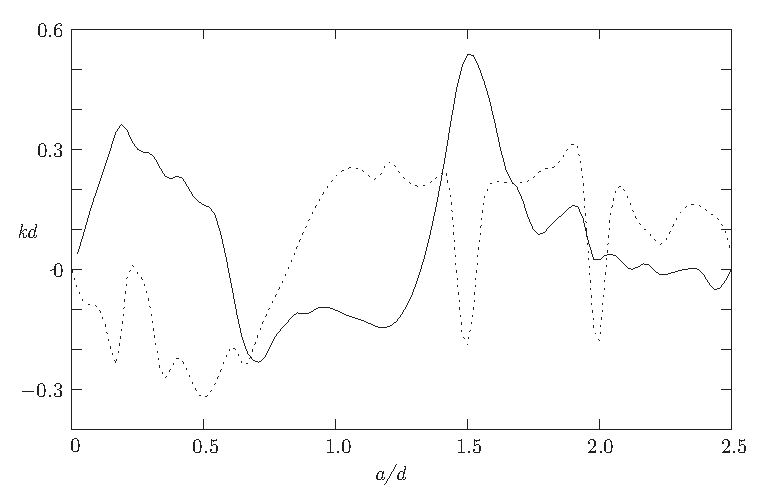
\includegraphics{trapped.eps}% Images in 100% size
  \caption{Trapped-mode wavenumbers, $kd$, plotted against $a/d$ for
    three ellipses:\protect\\%
    ---$\!$---,
    $b/a=1$; $\cdots$\,$\cdots$, $b/a=1.5$.}
\label{fig:ka}
\end{figure}

\begin{figure}
  \centering
  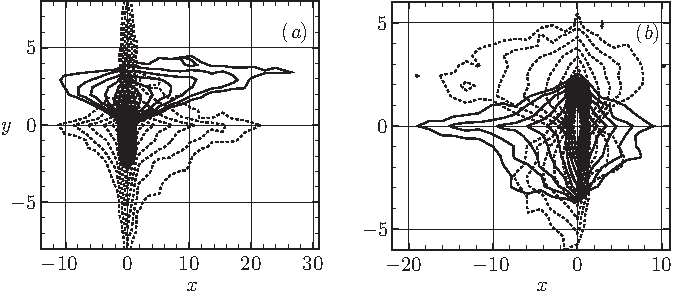
\includegraphics{modes}
  \caption{The features of the four possible modes corresponding to
  (\textit{a}) periodic\protect\\ and (\textit{b}) half-periodic solutions.}
\label{fig:kd}
\end{figure}

\subsection{Tables}
Tables, however small, must be numbered sequentially in the order in which they are mentioned in the text. The word \textit {table} is only capitalized at the start of a sentence. See table \ref{tab:kd} for an example.

\begin{table}
  \begin{center}
\def~{\hphantom{0}}
  \begin{tabular}{lccc}
      $a/d$  & $M=4$   &   $M=8$ & Callan \etal \\[3pt]
       0.1   & 1.56905 & ~~1.56~ & 1.56904\\
       0.3   & 1.50484 & ~~1.504 & 1.50484\\
       0.55  & 1.39128 & ~~1.391 & 1.39131\\
       0.7   & 1.32281 & ~10.322 & 1.32288\\
       0.913 & 1.34479 & 100.351 & 1.35185\\
  \end{tabular}
  \caption{Values of $kd$ at which trapped modes occur when $\rho(\theta)=a$}
  \label{tab:kd}
  \end{center}
\end{table}


\subsection{Datasets}
JPP encourages authors to make available the underlying dataset of their article. JPP has partnered with Zenodo to provide authors with the tools to do this. Zenodo is a free service that gives authors the ability to deposit and provide access to the data objects or datasets that underlie the figures and tables in their published research. Zenodo assigns all publically available uploads a DOI so that the datasets can be easily referenced. For further information and guidelines on how to deposit a dataset in Zenodo, please read the separate document JPP-Zenodo guide for authors.

\subsection{Online supplementary material}\label{online}
Relevant material which is not suitable for inclusion in the main article body, such as movies or numerical simulations/animations, can be uploaded as part of the initial submission. Each individual file must be accompanied by a separate caption and a suitable title (which can be provided in a Word file), such as `Movie 1', and large files should be archived as a .zip or .tar file before uploading. Each individual supplementary file should be no more than 10MB. Upon publication these materials will then be hosted online alongside the final published article. Likewise, should there be detailed mathematical relations, tables or figures which are likely to be useful only to a few specialists, these can also be published online as supplementary material. Note that supplementary material is published `as is', with no further production performed.

\section{Editorial decisions}

\subsection{Revision}
If a revision is requested, you should upload revised files following the same procedure as for submitting a new paper. You begin by clicking on `Manuscripts with decision' in your Corresponding Author Center, and then on `Create a revision'. (Note that if you abandon the process before completing the submission, to continue the submission, you must click on `Revised manuscripts in draft'.) There is a new first page showing the decision letter and a space for your reply to the referee's/editor's comments. You also have the opportunity at this stage to upload your reply to the comments as a separate file. All the values filled in on original submission are displayed again. The ID number of the paper will be appended `.R1'.

\subsection{Provisional acceptance}
If the paper is accepted as suitable for publication you will be sent a provisional acceptance decision. This enables you to upload the final files required for production:
\begin{enumerate}
\item the final PDF or Word version of the paper, designated as a `main document';
\item any source files (see section \ref{sec:filetypes}) which must be designated as `production (not for review)' and uploaded as a single .zip or .tar file.
\end{enumerate}

In the decision email a link to the transfer of copyright form will also be sent, and this form can either be uploaded with the files mentioned above, or can be sent separately. No paper can be published without a completed transfer of copyright form.

Please note JPP standard procedure is for authors to assign copyright to Cambridge University Press. For research funded by bodies which insist on retention of copyright (for example EURATOM), we can provide an alternative grant of licence form. 

\subsection{Acceptance}
On receipt of the production files you will be sent an email indicating completion of the acceptance process.

\section{Publication process}
Once a paper has been accepted for publication and the source files have been uploaded, the manuscript will be sent to Cambridge University Press for copyediting and typesetting, and will be assigned a digital object identifier (doi). When the proof is ready, authors will receive an email alert containing a link to the PDF of the proof, and instructions for its correction and return. It is imperative that authors check their proofs closely, particularly the equations and figures, which should be checked against the accepted file, as the production schedule does not allow for corrections at a later stage. Your JPP article will be published straight into an issue online as soon as it is ready. The PDF published online is the Version of Record and no further alterations/corrections to this document will be allowed.

\section{Obtaining help}
Technical support for the online submission system is available by clicking on the `Get Help Now' link at the top-right corner of each page of the submission site. Any other questions relating to the submission or publication process should be directed to the JPP Editorial Assistant, Mrs Amanda Johns, at plaeditorial@cambridge.org.

\section{Notation and style}\label{notstyle}
Generally any queries concerning notation and journal style can be answered by viewing recent pages in the Journal. However, the following guide provides the key points to note. It is expected that Journal style will be followed, and authors should take care to define all variables or entities upon first use. Also note that footnotes are not normally accepted.

\subsection{Mathematical notation}
\subsubsection{Setting variables, functions, vectors, matrices etc}

\textbf{Italic font} should be used for denoting variables, with multiple-letter symbols avoided except in the case of dimensionless numbers.

\textbf{Upright Roman font} (or upright Greek where appropriate) should be used for:
\begin{itemize}
\item Operators: sin, log, d, $\Delta$, e etc.
\item Constants: i ($\sqrt{-1}$), $\upi$ (defined as \verb}\upi}), etc.
\item Functions: $\Ai$, $\Bi$ (Airy functions, defined as \verb|\Ai| and \verb|\Bi|), $\Real$ (real part, defined as \verb|\Real|), $\Imag$ (imaginary part, defined as \verb|\Imag|), etc.
\item Physical units: cm, s, etc
\item Abbreviations: c.c. (complex conjugate), h.o.t. (higher-order terms), DNS, etc.
\end{itemize}

\textbf{Bold italic font} (or bold sloping Greek) should be used for:

\begin{itemize}
\item  Vectors (with the centred dot for a scalar product also in bold): $\boldsymbol{i \cdot j}$
\end{itemize}

\textbf{Bold sloping sans serif font}, defined by the \verb|\mathsfbi| macro, should be used for:
\begin{itemize}
\item Tensors and matrices: $\mathsfbi{D}$
\end{itemize}

\textbf{Script font} (for example $\mathcal{G}$, $\mathcal{R}$) can be used as an alternative to italic when the same letter denotes a different quantity (use \verb|mathcal| in \LaTeX).

The product symbol ($\times$) should only be used to denote multiplication where an equation is broken over more than one line, to denote a cross product, or between numbers (the $\cdot$ symbol should not be used, except to denote a scalar product specifically).


\subsubsection{Other symbols}
A centred point should be used only for the scalar product of vectors.
Large numbers that are not scientific powers should not include commas, but have the
form 1600 or 16~000 or 160~000.
Use \textit{O} to denote `of the order of', not the \LaTeX\ $\mathcal{O}$.

\section{Citations and references}

%All papers included in the References section must be cited in the article, and vice versa. Citations should be included as, for example ``It has been shown \citep{Rogallo81} that...'' (using the {\verb}\citep} command, part of the natbib package) ``recent work by \citet{Dennis85}...'' (using {\verb}\citet}).
The natbib package can be used to generate citation variations, as shown below.
\cite{wenThunderGBMFastGBDTs}

% \begin{itemize}
% \item \verb#\citet[pp. 2-4]{Galtier00}#:
% \citet[pp. 479-480]{Galtier00} 
% \item \verb#\citep[p. 6]{Worster92}#:
% \citep[p. 6]{Worster92}
% \item \verb#\citep[see][]{Koch83, Lee71, Linton92}#:
% \citep[see][]{Koch83, Lee71, Linton92}
% \item \verb#\citep[see][p. 18]{Martin80}#:
% \citep[see][p. 18]{Martin80}
% \item \verb#\citep{Brownell04,Brownell07,Ursell50,Wijngaarden68,Miller91}#:
% \citep{Brownell04,Brownell07,Ursell50,Wijngaarden68,Miller91}
% \end{itemize}

The References section can either be built from individual \verb#\bibitem# commands, or can be built using BibTex. The BibTex files used to generate the references in this document can be found in the zip file in the Instructions for Contributors section of the JPP website.

Where there are up to ten authors, all authors' names should be given in the reference list. Where there are more than ten authors, only the first name should appear, followed by et al.

Acknowledgements should be included at the end of the paper, before the References section or any appendicies, and should be a separate paragraph without a heading. Several anonymous individuals are thanked for contributions to these instructions.

\appendix

\section{}\label{appA}
This appendix contains sample equations in the JPP style. Please refer to the {\LaTeX} source file for examples of how to display such equations in your manuscript.

\begin{equation}
  (\nabla^2+k^2)G_s=(\nabla^2+k^2)G_a=0
  \label{Helm}
\end{equation}

\begin{equation}
  \bnabla\bcdot\boldsymbol{v} = 0,\quad \nabla^{2}P=
    \bnabla\bcdot(\boldsymbol{v}\times \boldsymbol{w}).
\end{equation}

\begin{equation}
  G_s,G_a\sim 1 / (2\upi)\ln r
  \quad \mbox{as\ }\quad r\equiv|P-Q|\rightarrow 0,
  \label{singular}
\end{equation}

\begin{equation}
\left. \begin{array}{ll}  
\displaystyle\frac{\p G_s}{\p y}=0
  \quad \mbox{on\ }\quad y=0,\\[8pt]
\displaystyle  G_a=0
  \quad \mbox{on\ }\quad y=0,
 \end{array}\right\}
  \label{symbc}
\end{equation}


\begin{equation}
  -\frac{1}{2\upi} \int_0^{\infty} \gamma^{-1}[\mathrm exp(-k\gamma|y-\eta|)
   + \mathrm exp(-k\gamma(2d-y-\eta))] \cos k(x-\xi)t\:\mathrm{d} t,
   \qquad 0<y,\quad \eta<d,
\end{equation}

\begin{equation}
  \gamma(t) = \left\{
    \begin{array}{ll}
      -\mathrm{i}(1-t^2)^{1/2}, & t\le 1 \\[2pt]
      (t^2-1)^{1/2},         & t>1.
    \end{array} \right.
\end{equation}

\[
  -\frac{1}{2\upi}
   \pvi B(t)\frac{\cosh k\gamma(d-y)}{\gamma\sinh k\gamma d}
   \cos k(x-\xi)t\:\mathrm{d} t
\]

\begin{equation}
  G = -\frac{1}{4}\mathrm{i} (H_0(kr)+H_0(kr_1))
    - \frac{1}{\upi} \pvi\frac{\mathrm{e}^{-\kgd}}%
    {\gamma\sinh\kgd} \cosh k\gamma(d-y) \cosh k\gamma(d-\eta)
\end{equation}

Note that when equations are included in definitions, it may be suitable to render them in line, rather than in the equation environment: $\boldsymbol{n}_q=(-y^{\prime}(\theta),
x^{\prime}(\theta))/w(\theta)$.
Now $G_a=\squart Y_0(kr)+\Gat$ where
$r=\{[x(\theta)-x(\psi)]^2 + [y(\theta)-y(\psi)]^2\}^{1/2}$ and $\Gat$ is
regular as $kr\ttz$. However, any fractions displayed like this, other than $\thalf$ or $\squart$, must be written on the line, and not stacked (ie 1/3).
 
\begin{align}
  \ndq\left(\frac{1}{4} Y_0(kr)\right) & \sim 
    \frac{1}{4\upi w^3(\theta)}
    [x^{\prime\prime}(\theta)y^{\prime}(\theta)-
    y^{\prime\prime}(\theta)x^{\prime}(\theta)] \nonumber\\
  & =  \frac{1}{4\upi w^3(\theta)}
    [\rho^{\prime}(\theta)\rho^{\prime\prime}(\theta)
    - \rho^2(\theta)-2\rho^{\prime 2}(\theta)]
    \quad \mbox{as\ }\quad kr\ttz . \label{inteqpt}
\end{align}

\begin{equation}
  \frac{1}{2}\phi_i = \frac{\upi}{M} \sumjm\phi_j K_{ij}^a w_j,
  \qquad i=1,\,\ldots,\,M,
\end{equation}
where
\begin{equation}
  K_{ij}^a = 
      \begin{cases}
      \p G_a(\theta_i,\theta_j)/\p n_q, & i\neq j \\[2pt]
      \p\Gat(\theta_i,\theta_i)/\p n_q
      + [\rho_i^{\prime}\rho_i^{\prime\prime}-\rho_i^2-2\rho_i^{\prime 2}]
      / 4\upi w_i^3, & i=j.
      \end{cases}
\end{equation}


\refstepcounter{equation}
\[
  \rho_l = \lim_{\zeta \rightarrow Z^-_l(x)} \rho(x,\zeta), \quad
  \rho_{u} = \lim_{\zeta \rightarrow Z^{+}_u(x)} \rho(x,\zeta)
  \eqno{(\theequation{\mathit{a},\mathit{b}})}\label{eq35}
\]

\begin{equation}
  (\rho(x,\zeta),\phi_{\zeta\zeta}(x,\zeta))=(\rho_0,N_0)
  \quad \mbox{for}\quad Z_l(x) < \zeta < Z_u(x).
\end{equation}


\begin{subeqnarray}
  \tau_{ij} & = &
    (\overline{\overline{u}_i \overline{u}_j}
    - \overline{u}_i\overline{u}_j)
    + (\overline{\overline{u}_iu^{SGS}_j
    + u^{SGS}_i\overline{u}_j})
    + \overline{u^{SGS}_iu^{SGS}_j},\\[3pt]
  \tau^\theta_j & = &
    (\overline{\overline{u}_j\overline{\theta}}
    - \overline{u}_j \overline{\theta})
    + (\overline{\overline{u}_j\theta^{SGS}
    + u^{SGS}_j \overline{\theta}})
    + \overline{u^{SGS}_j\theta^{SGS}}.
\end{subeqnarray}

\begin{equation}
\setlength{\arraycolsep}{0pt}
\renewcommand{\arraystretch}{1.3}
\slsQ_C = \left[
\begin{array}{ccccc}
  -\omega^{-2}V'_w  &  -(\alpha^t\omega)^{-1}  &  0  &  0  &  0  \\
  \displaystyle
  \frac{\beta}{\alpha\omega^2}V'_w  &  0  &  0  &  0  &  \mathrm{i}\omega^{-1} \\
  \mathrm{i}\omega^{-1}  &  0  &  0  &  0  &  0  \\
  \displaystyle
  \mathrm{i} R^{-1}_{\delta}(\alpha^t+\omega^{-1}V''_w)  &  0
    & -(\mathrm{i}\alpha^tR_\delta)^{-1}  &  0  &  0  \\
  \displaystyle
  \frac{\mathrm{i}\beta}{\alpha\omega}R^{-1}_\delta V''_w  &  0  &  0
    &  0  & 0 \\
  (\mathrm{i}\alpha^t)^{-1}V'_w  &  (3R^{-1}_{\delta}+c^t(\mathrm{i}\alpha^t)^{-1})
    &  0  &  -(\alpha^t)^{-2}R^{-1}_{\delta}  &  0  \\
\end{array}  \right] .
\label{defQc}
\end{equation}

\begin{equation}
\etb^t = \skew2\hat{\etb}^t \exp [\mathrm{i} (\alpha^tx^t_1-\omega t)],
\end{equation}
where $\skew2\hat{\etb}^t=\boldsymbol{b}\exp (\mathrm{i}\gamma x^t_3)$. 
\begin{equation}
\mbox{Det}[\rho\omega^2\delta_{ps}-C^t_{pqrs}k^t_qk^t_r]=0,
\end{equation}

\begin{equation}
 \langle k^t_1,k^t_2,k^t_3\rangle = \langle
\alpha^t,0,\gamma\rangle  
\end{equation}

\begin{equation}
\boldsymbol{f}(\theta,\psi) = (g(\psi)\cos \theta,g(\psi) \sin \theta,f(\psi)).
\label{eq41}
\end{equation}

\begin{eqnarray}
f(\psi_1) = \frac{3b}{\upi[2(a+b \cos \psi_1)]^{{3}/{2}}}
  \int^{2\upi}_0 \frac{(\sin \psi_1 - \sin \psi)(a+b \cos \psi)^{1/2}}%
  {[1 - \cos (\psi_1 - \psi)](2+\alpha)^{1/2}}\mathrm{d}x,
\label{eq42}
\end{eqnarray}
\begin{eqnarray}
g(\psi_1) & = & \frac{3}{\upi[2(a+b \cos \psi_1)]^{{3}/{2}}}
  \int^{2\upi}_0 \left(\frac{a+b \cos \psi}{2+\alpha}\right)^{1/2}
  \left\{ \astrut f(\psi)[(\cos \psi_1 - b \beta_1)S + \beta_1P]
  \right. \nonumber\\
&& \mbox{}\times \frac{\sin \psi_1 - \sin \psi}{1-\cos(\psi_1 - \psi)}
  + g(\psi) \left[\left(2+\alpha - \frac{(\sin \psi_1 - \sin \psi)^2}
  {1- \cos (\psi - \psi_1)} - b^2 \gamma \right) S \right.\nonumber\\
&& \left.\left.\mbox{} + \left( b^2 \cos \psi_1\gamma -
  \frac{a}{b}\alpha \right) F(\frac{1}{2}\upi, \delta) - (2+\alpha)
  \cos\psi_1 E(\frac{1}{2}\upi, \delta)\right] \astrut\right\} \mathrm{d} \psi,
\label{eq43}
\end{eqnarray}
\begin{equation}
\alpha = \alpha(\psi,\psi_1) = \frac{b^2[1-\cos(\psi-\psi_1)]}%
  {(a+b\cos\psi) (a+b\cos\psi_1)},
  \quad
  \beta - \beta(\psi,\psi_1) = \frac{1-\cos(\psi-\psi_1)}{a+b\cos\psi}.
\end{equation}


\begin{equation}
\left. \begin{array}{l}
\displaystyle
H(0) = \frac{\epsilon \overline{C}_v}{\tilde{v}^{{1}/{2}}_T
(1- \beta)},\quad H'(0) = -1+\epsilon^{{2}/{3}} \overline{C}_u
+ \epsilon \skew5\hat{C}_u'; \\[16pt]
\displaystyle
H''(0) = \frac{\epsilon u^2_{\ast}}{\tilde{v}^{{1}/{2}}
_T u^2_P},\quad H' (\infty) = 0.
\end{array} \right\}
\end{equation}




\begin{lemma}

%\citet[][pp.~231--232]{Batchelor59}

Let $f(z)$ be a trial  function defined on $[0,1]$.  Let $\varLambda_1$ denote
the ground-state eigenvalue for $-\mathrm{d}^2g/\mathrm{d} z^2=\varLambda g$,
where $g$ must satisfy $\pm\mathrm{d} g/\mathrm{d} z+\alpha g=0$ at $z=0,1$
for some non-negative constant~$\alpha$.  Then for any $f$ that is not
identically zero we have
\begin{equation}
\frac{\displaystyle
  \alpha(f^2(0)+f^2(1)) + \int_0^1 \left(
  \frac{\mathrm{d} f}{\mathrm{d} z} \right)^2 \mathrm{d} z}%
  {\displaystyle \int_0^1 f^2\mathrm{d} z}
\ge \varLambda_1 \ge
\left( \frac{-\alpha+(\alpha^2+8\upi^2\alpha)^{1/2}}{4\upi} \right)^2.
\end{equation}
\end{lemma}



\begin{corollary}
Any non-zero trial function $f$ which satisfies the boundary condition
$f(0)=f(1)=0$ always satisfies
\begin{equation}
  \int_0^1 \left( \frac{\mathrm{d} f}{\mathrm{d} z} \right)^2 \mathrm{d} z.
\end{equation}
\end{corollary}

% susie put cite commands here, don't bother with citet etc just yet.

% \bibliographystyle{jpp}
% \bibliographystyle{IEEEtran}
% Note the spaces between the initials



% \bibliography{jpp-instructions}
\printbibliography


\end{document}
